% Retained mathematical and signed-error diagnostics from the earlier main text.
\subsection{Restricted information analysis}
For fixed point-to-plane correspondences and small pure translation,
\begin{equation}
b=A\Delta x+\epsilon,\qquad j=d^T\Delta x.
\end{equation}
\begin{proposition}
The noiseless task scalar is identifiable for every displacement iff
$d\in\operatorname{range}(A^T)$. When identifiable, minimum-norm exact weights are
$\ell=A(A^TA)^\dagger d$, and
$|\ell^Tb-j|\leq\norm{\ell}\norm{\epsilon}$.
\end{proposition}
\noindent\emph{Proof:} Indistinguishable translations differ by $z\in\ker A$; their task scalars agree iff $d^Tz=0$ for every such $z$. Exact weights satisfy $A^T\ell=d$; the minimum-norm solution is as stated, and Cauchy--Schwarz gives the bound.\hfill$\square$

This standard fact excludes uncertain normals, incorrect association, rotation and evolving maps. A circle's absolute rotation ambiguity does not imply that its translation is unidentifiable. Polygon discretization is part of our executed model. The earlier synthetic observation-layout test is preserved as supplementary diagnosis; no new sensing policy is evaluated in the census.

The rejected candidate reads
\begin{equation}
\widehat J^{a}_k=g\bigl(d^Tm_k^-+\ell_k^Tb_k\bigr),\qquad g=1.24.
\end{equation}
It retains the historical map anchor. Under the restrictive rigid-map residual model
$b_k=A_k[(x_k-x_0)-m_k^-]+\eta_k$,
its error is $(g-1)J_k+g\ell_k^T\eta_k$.
A correct certificate does not remove the gain term or bound real map/correspondence errors. This equation is a limitation, not evidence that gain alone caused the observed failures.

\subsection{Signed cumulative accounting from existing logs}
The offline audit uses the recorded pre-physics control-time truth. For robot $i$, define $u_{ik}=d^Tm^+_{ik}$, held-readout term
$h_{ik}=r^{\rm original}_{ik}-gu_{ik}$, and candidate term
$c_{ik}=r_{ik}-r^{\rm original}_{ik}$. Then
$r_{ik}=u_{ik}+(g-1)u_{ik}+h_{ik}+c_{ik}$.
Median weights $w_{ik}$ reproduce actual team progress $T_k$; tied values use an explicit agent-ID rule. The component allocation is not unique at ties and is not a causal attribution.

With $E_k=T_k-J_k$,
\begin{align}
\Delta E_k={}&\sum_iw_{ik}(\Delta u_{ik}-\Delta J_k)
+\sum_iw_{ik}(g-1)\Delta u_{ik}\nonumber\\
&+\sum_iw_{ik}\Delta h_{ik}+\sum_iw_{ik}\Delta c_{ik}
+\sum_i\Delta w_{ik}r_{i,k-1}.
\end{align}
Accumulating all terms and the initial error reconstructs the signed error; omitting the voter-change term would misallocate it. Registration plus fusion also reconstructs map increments to numerical precision. Both are accounting checks, not physical-estimation proofs.

\begin{table}[t]
\caption{Baseline cumulative signed-error accounting, millimeters, at the last aligned control instant. Components use a fixed median tie rule and are not causal effects. Displayed terms are rounded.}
\centering\footnotesize
\begin{tabular}{lrrrrr}\toprule
Case & Map--truth & Gain & Held & Voters & Total\\\midrule
R2 & -18.9 & 306.0 & -13.9 & -102.4 & 170.8 \\
L8 & -168.7 & 236.4 & 36.6 & 50.7 & 154.9 \\
C8 & -240.0 & 255.7 & 22.5 & -2.1 & 36.0 \\
\bottomrule\end{tabular}
\end{table}
The residual of cumulative reconstruction is below $10^{-12}$ m in every arm. The different signed terms can compensate or reinforce each other; they do not isolate an implementation defect. The raw-map, gain, hold and endogenous voter effects remain hypotheses for future targeted tests, not a reason to tune this completed batch.


For the v2 baseline episodes, the first shared HOLD in rectangle and L occurs with true speeds zero but endpoint errors outside the original task tolerance. Estimated/true progress is $1.4651/1.2939$ m against $L=1.4467$ m for rectangle, and $1.3082/1.1535$ m against $L=1.3044$ m for L. C has already reached the projected goal. These observations identify premature spatial stopping in the selected failures. Individual transport-loop hysteretic holding states were not saved; their exact first transitions cannot be reconstructed from scalar input alone. No new gain, certificate or candidate is introduced.


\begin{figure*}[t]
\centering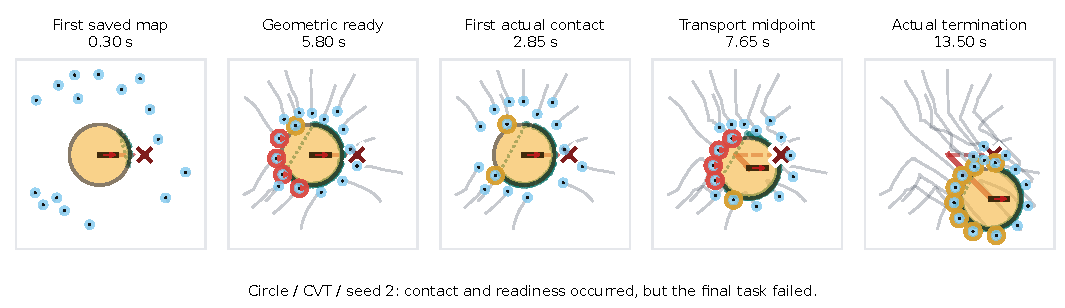
\includegraphics[width=\textwidth]{generated/media_v1/full_process.pdf}
\caption{Circle/CVT event-indexed process: first saved local map, geometric readiness, first physical contact, transport midpoint and actual termination. Event columns need not be chronological: contact here precedes readiness. Orange is evaluation geometry, teal is agent 00's fused map, and rings mark geometric readiness, not contact. The final task fails despite G500 passing.}
\label{fig:process}
\end{figure*}
